\clearpage

\section{Probability and measure theory}

This section contains the prerequisites of measure-theoric view of probability.
It is not a full recount of the theory, it only has bits and pieces as and when needed.

\begin{notebox}
Based mainly on \fullcite{siegristRandomProbabilityMathematical}

\hfill Notes taken: endJan - earlyFeb 2020 \index{February 2020}
\end{notebox}

%%%%%%%%%%%%%%%%%%%%%%%%%%%%%%%%%%%%%%%%%%%%%%%%%%%%%%
%%%%%%%%%%%%%%%%% Measure theory %%%%%%%%%%%%%%%%%%%%%
%%%%%%%%%%%%%%%%%%%%%%%%%%%%%%%%%%%%%%%%%%%%%%%%%%%%%%
\subsection{Measure theory}

\subsubsection{Measurable space}

\begin{definition}
A \textbf{$\sigma$-algebra}\index{$\sigma$-algebra} $\mathscr{S}$ of a set $S$ is a \emph{non-empty} collection of subsets of $S$ that is closed under a \emph{countable} number of set operations.
That is:
\begin{compactitem}
\item if $A \in \mathscr{S}$ then $A^c \in \mathscr{S}$
\item if $A_i \in \mathscr{S}$ for each $i$ in a countable index set $I$ then $\cup_{i \in I} A_i \in \mathscr{S}$.
\end{compactitem}
\end{definition}

Additional properties of \textbf{$\sigma$-algebra} $\mathscr{S}$
\begin{compactitem}
\item $S \in \mathscr{S}$ \hspace{0.5cm}
(Proof: For any $A \in \mathscr{S}$, we have $A^c \in \mathscr{S}$ and $S = A \cup A^c \in \mathscr{S}$.)
\item $\emptyset \in \mathscr{S}$ \hspace{0.5cm}
(Proof: From above $S \in \mathscr{S}$ and $S^c = \emptyset \in \mathscr{S}$.)
\item if $A_i \in \mathscr{S}$ for each $i$ in a countable index set $I$ then $\cap_{i \in I} A_i \in \mathscr{S}$ \hspace{0.5cm}
(Proof: If $A_i \in \mathscr{S}$ then $A_i^c \in \mathscr{S}$ and since $B = \cup_{i \in I} A_i^c \in \mathscr{S}$ then $B^c = \cap_{i \in I} A_i \in \mathscr{S}$.)
\end{compactitem}

\begin{definition}
A \textbf{measurable space}\index{measurable space} is the space $(S, \mathscr{S})$ consisting of a set $S$,  and the $\sigma$-algebra $\mathscr{S}$.
\end{definition}

\begin{definition}
A \textbf{Borel $\sigma$-algebra}\index{Borel $\sigma$-algebra} is the algebra $\sigma(\mathscr{S})$ generated by the open sets of the topological space $(S, \mathscr{S})$.

Note: Since closed sets are complements of open sets, the Borel $\sigma$-algebra contains the closed sets as well (and is in fact generated by the closed sets).
\end{definition}

\subsubsection{Measurable function}

\begin{definition}
Suppose sets $S$ and $T$ and a function $f : S \to T$.
If $A \subseteq T$, the \textbf{inverse image (pre-image)}\index{inverse image}\index{pre-image} of A under f is the subset of $S$ given by $f^{-1}(A) = \{x \in S : f(x) \in A\}$.

Note: Careful, though the notation is the same, the inverse image does not have to be a function (the inverse function may not exist).
\end{definition}

\begin{definition}
Suppose sets $S$ and $T$ and a function $f : S \to T$.
If $A \subseteq S$, the \textbf{forward (direct) image}\index{forward image}\index{direct image} of A under f is the subset of $T$ given by $f(A) = \{f(x) \in T : x \in A\}$.
\end{definition}

\begin{definition}
A \textbf{measurable function}\index{measurable function} is a function $f: S \to T$ where $(S, \mathscr{S})$ and $(T, \mathscr{T})$ are measurable spaces and $f^{-1}(A) \in \mathscr{S}$ for any $A \in \mathscr{T}$.

Note: a continuous function $f: S \to T$ is measurable.
\end{definition}

\subsubsection{Measure}

\begin{definition}
A \textbf{positive measure}\index{positive measure} on $(S, \mathscr{S})$ is the function $\mu : \mathscr{S} \to [0, \infty]$ such that:
\begin{compactitem}
\item $\mu(\emptyset) = 0$
\item if $\{A_i : i \in I \}$ is a countable, pairwise disjoint collection of sets on $\mathscr{S}$ then $\mu(\cup_{i \in I} A_i) = \sum_{i \in I} \mu(A_i)$ ($\sim$ \emph{countable additivity}\index{countable additivity}). 
\end{compactitem}
The triple $(S, \mathscr{S}, \mu)$ is a \textbf{measure space}\index{measure space}.
\end{definition}

\begin{theorem}[Push-forward measure]\index{push-forward measure}
Assume a measure space $(S, \mathscr{S}, \mu)$ a measurable space $(T, \mathscr{T})$ and a measurable function $f : S \to T$.
Then $\nu$ defined as below is a positive measure on $(T, \mathscr{T})$
\begin{equation*}
\nu(B) = \mu(f^{-1}(B)), \quad B \in \mathscr{T}
\end{equation*}
\end{theorem}

\begin{figure}[ht]
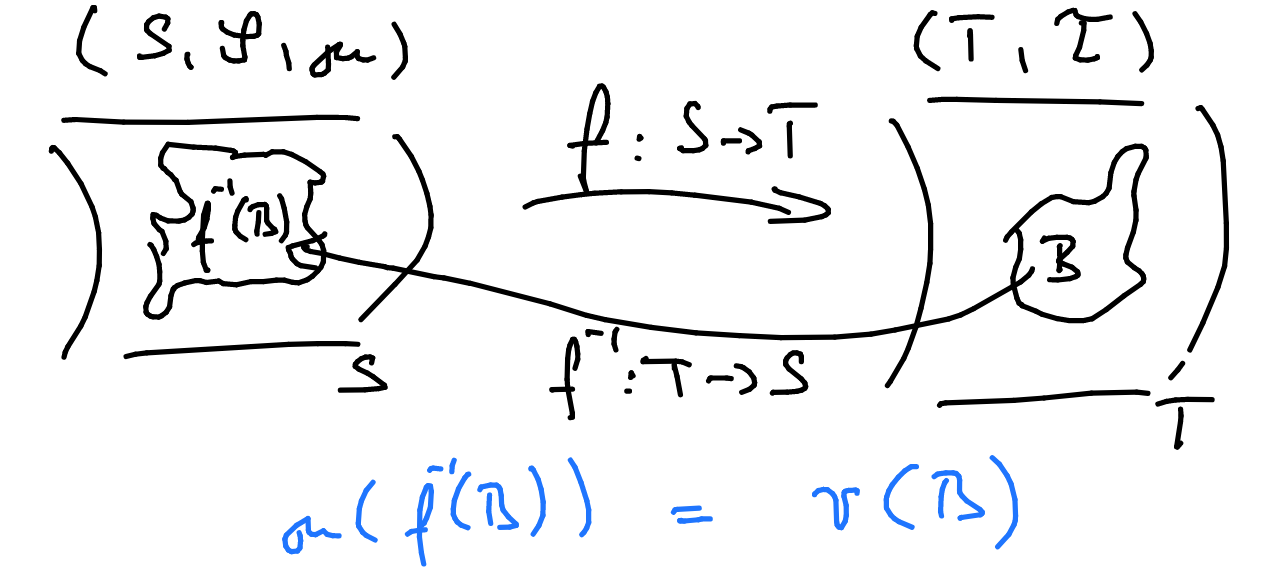
\includegraphics[width=0.5\textwidth]{changeOfVar}
\centering
\end{figure}

\begin{definition}
A \textbf{null set}\index{null set} of a measure space $(S, \mathscr{S}, \mu)$ is the set $A \in \mathscr{S}$ such that $\mu(A) = 0$.
\end{definition}

\begin{definition}
Consider a statement with $x \in S$ as a free variable.
\begin{compactitem}
\item The statement \textbf{holds on} $A$ if it is true for every $x \in A$
\item The statement \textbf{holds almost everywhere on} $A$\index{almost everywhere} (with respect to $\mu$) if there exists $B \in \mathscr{S}$ with $B \subseteq A$ such that the statement holds on B and $\mu(A \backslash B) = 0$ (\emph{null set}).
\end{compactitem}
\end{definition}


\begin{definition}
Sets $A, B \in \mathscr{S}$ are \textbf{equivalent}\index{equivalent sets} ($A \equiv B$) if $\mu(A \backslash B) + \mu(B \backslash A) = 0$ (the set of elements in which these two differ has measure zero).

Two measurable functions $f, g : S \to T$ are equivalent if $\mu\{x \in S : f(x) \neq g(x)\} = 0$ (the functions are only different over a set of x with measure zero).
\end{definition}

\begin{definition}
Suppose $\mu$ and $\nu$ are measures on $(S, \mathscr{S})$
\begin{compactenum}[a.]
\item $\nu$ is \textbf{absolutely continuous}\index{absolutely continuous measure} with respect to $\mu$ if every null set of $\mu$ is also a null set of $\nu$. We write $\nu \ll \mu$.
\item $\nu$ and $\mu$ are \textbf{mutually singular}\index{mutually singular measures} if there exists $A \in \mathscr{S}$ such that $A$ is null for $\mu$ and $A^c$ is null for $\nu$. We write $\mu \perp \nu$.
\item $\nu$ and $\mu$ are \textbf{equivalent}\index{equivalent measures} if $\mu \ll \nu$ and $\nu \ll \mu$. We write $\mu \equiv \nu$.
\end{compactenum}
\end{definition}

%%%%%%%%%%%%%%%%%%%%%%%%%%%%%%%%%%%%%%%%%%%%%%%%%%%%%%
%%%%%%%%%%%%%% Some standard measures %%%%%%%%%%%%%%%%
%%%%%%%%%%%%%%%%%%%%%%%%%%%%%%%%%%%%%%%%%%%%%%%%%%%%%%
\subsubsection{Some standard measures}

\paragraph{Borel measure}

\begin{definition}
A topological space $(S, \mathscr{T})$ with $\mathscr{S} = \sigma(\mathscr{T})$ a Borel $\sigma$-algebra has a positive measure $\mu$ on $(S, \mathscr{S})$ called the \textbf{Borel measure}\index{Borel measure}. The triplet $(S, \mathscr{S}, \mu)$ is a \textbf{Borel measure space}\index{Borel measure space}.
\end{definition}

\paragraph{Lebesgue measure}

\begin{definition}[Lebesgue measure]
For the standard \emph{Euclidean space} $(\mathbb{R}, \mathscr{R})$, $\mathscr{R}$ is the Borel $\sigma$-algebra generated by the standard Euclidean topology (collection of open or closed intervals $\mathscr{I}$ on $\mathbb{R}$).

For $a \leq b \in \mR$ all of the intervals $(a, b), (a, b], [a, b), [a, b]$ have the same \textbf{length} $b-a$.
Intervals $(a, \infty), [a, \infty), (-\infty, a), (-\infty, a]$ have all \textbf{length} $\infty$ and so does $\mR$ itself.

There exists a unique measure $\lambda$ on $\mathscr{R}$ such that $\lambda(I) = length(I)$ for all $I \in \mathscr{I}$.
This is the \textbf{Lebesgue measure}\index{Lebesgue measure} on $(\mathbb{R}, \mathscr{R})$.
\end{definition}

\begin{definition}[Lebesgue measure]
In the \emph{n-dimensional Euclidean space} $(\mathbb{R}^n, \mathscr{R}_n)$, the $\sigma$-algebra $\mathscr{R}_n$ is the n-fold power of $\mathscr{R}$, the Borel $\sigma$-algebra on $\mR$.
That is $\mathscr{R}_n = \mathscr{R} \otimes \mathscr{R} \otimes \ldots \otimes \mathscr{R}$.
It is also the sigma algebra generated by the products of intervals $\mathscr{R}_n = \sigma\{I_1 \times I_2 \times \ldots \times I_n : I_j \in \mathscr{I}, j \in \{1, 2, \dots, n\} \}$.

For $n \in \mN_+$ the n-fold power of $\lambda$ denoted $\lambda_n$ is the \textbf{Lebesgue measure} on $(\mathbb{R}^n, \mathscr{R}_n)$. In particular $\lambda(A_1 \times A_2 \times \ldots \times A_n) = \lambda(A_1) \lambda(A_2) \cdots \lambda(A_n); \ A_1, \ldots, A_n \in \mathscr{R}$ so that $\lambda_n$ is the \emph{n-dimensional volume} of $A \in \mathscr{R}_n$.
\end{definition}

Note: important properties of Lebesgue measure:
\begin{description}
\item[Translation invariance] If $A \subset \mR^n$ and $h \in \mR^n$ then $A + h \subseteq \mR^n$ and $\lambda_n(A) = \lambda_n(A + h)$
\item[Linear transformation] For linear map $T : \mR^n \to \mR^n$ and $A \subseteq \mR^n$ we denote by $TA = \{Tx \in \mR^n : x \in A\}$. Then $\lambda_n(TA) = \abs{\det T} \, \lambda_n(A)$ (by the usual interpretation of determinant as measuring the scaling of the linear transformation).
\item[Nonlinear differentiable transformation] For differentiable map $f : \mR^n \to \mR^n$ and $A \subseteq \mR^n$ we denote by $f(A) = \{f(x) \in \mR^n : x \in A\}$. Then $\lambda_n(f(A)) = \abs{\det J_f} \, \lambda_n(A)$ where $J_f = d f_i / d x_j$ is the Jacobian matrix. (This is probably not quite precise - Jacobian evaluated at which point as a local linear approximation?)
\end{description}


\paragraph{Lebesgue-Stieltjes measure}

\begin{definition}
A function $F : \mR \to \mR$  that satisfies
\begin{compactitem}
\item $F$ is increasing: if $x \leq y$ then $F(x) \leq F(y)$
\item $F$ is continuous from the right: $\lim_{t \downarrow x} F(t) = F(x)$ for all $x \in \mR$
\end{compactitem}
is a \textbf{distribution function}\index{distribution function} on $\mR$.
\end{definition}

\begin{definition}
If $F$ is a distribution function on $\mR$ then there exists a unique measure $\mu$ on $\mathscr{R}$ that satisfies $\mu(a, b] = F(b) - F(a), \ -\infty \leq a \leq b \leq \infty$. It is called the \textbf{Lebesgue-Stieltjes measure}\index{Lebesgue-Stieltjes measure}.
\end{definition}

\paragraph{Counting measure}

\begin{definition}
Assume a finite set $S$ with a power set (set of all subsets) $\mathscr{P}(S)$.
For $A \subseteq S$, the cardinality $\#(A)$ is the number of elements in $A$. The function $\#$ on $\mathscr{P}(S)$ is called the \textbf{counting measure}\index{counting measure}. (It is the usual measure on discrete spaces.)
\end{definition}

\paragraph{Probability measure}

\begin{definition}\label{defpre:probMeasure}
Suppose a measurable space $(S, \mathscr{S})$. 
A \textbf{probability measure}\index{probability measure} $\mP$ is a \emph{positive measure} on $(S, \mathscr{S})$ such that $\mP(S) = 1$.

%%%%%%%%%%%%%%%%%%%%%%%%%%%%%%%%%%%%%%%%%%%%%%%%%%%%%%
%%%%%%%%%%%%%%%%%%%%%% Probability %%%%%%%%%%%%%%%%%%%
%%%%%%%%%%%%%%%%%%%%%%%%%%%%%%%%%%%%%%%%%%%%%%%%%%%%%%
\subsection{Probability space}


\begin{definition}
A \textbf{probability space}\index{probability space} $(S, \mathscr{S}, \mathbb{P})$ consists of a set of outcomes of a random experiment $S$, the $\sigma-$algebra of events $\mathscr{S}$, and the probability measure $\mathbb{P}$ on the sample space $(S, \mathscr{S})$.

Note: $(\Omega, \mathscr{F}, \mP)$ is often used as special notation for probability spaces 
\end{definition}


Note: Any finite positive measure $\mu$ on the sample space $(S, \mathscr{S})$ can be re-scaled into a probability measure as $\mP(A) = \mu(A) / \mu(S), \ A \in \mathscr{S}$.

Note: Probability measure and \textbf{probability distribution}\index{probability distribution} are equivalent terms.
\end{definition}

\begin{definition}[random variable]
Suppose that $(S, \mathscr{S}, \mathbb{P})$ is a probability space and $(T, \mathscr{T})$ is another measurable space.
A \textbf{random variable}\index{random variable} $X$ with values in $T$ is a \emph{measurable} function from $S$ to $T$ ($X: S \to T$).
\begin{compactitem}
\item the probability measure of $X$ (the \emph{probability distribution} of $X$) is the mapping $P : T \to [0, 1]$ given by $P : B \to \mP(X \in B)$ (push-forward measure).
\item the collection of events $\{ X \in B : B \in \mathscr{T} \}$ is a sub $\sigma$-algebra of $\mathscr{S}$ and it is the $\sigma$-algebra generated by $X$ denoted by $\sigma(X)$
\end{compactitem}
Note: measurability of $X$ ensure that the inverse image of $B$ under $X$ (that is $\{X \in B\} = \{s \in S : X(s) \in B\}$) is in $\mathscr{S}$ (and hence is a valid event in $S$) for all $B \in \mathscr{T}$.
\end{definition}

\begin{figure}[ht]
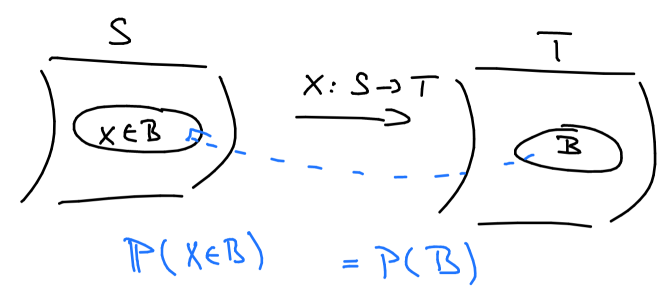
\includegraphics[width=0.5\textwidth]{probOfRV}
\centering
\end{figure}

\begin{definition}
Suppose that $(S, \mathscr{S}, \mathbb{P})$ is a probability space. 
Define the following collections of events
\begin{compactitem}
\item $\mathcal{N} = \{A \in \mathscr{S} : \mP(A) = 0\}$, the collection of \textbf{null} events\index{null events}
\item $\mathcal{M} = \{A \in \mathscr{S} : \mP(A) = 1\}$, the collection of \textbf{almost sure} events\index{almost sure events}
\item $\mathcal{D} = \mathcal{N} \bigcup \mathcal{M} = \{A \in \mathscr{S} : \mP(A) = 0 or \mP(A) = 1\}$, the collection of \textbf{essentially deterministic} events\index{essentially deterministic events}
\end{compactitem}
The collection of essentially deterministic events $\mathcal{D}$ is a sub $\sigma$-algebra of $\mathscr{S}$.
\end{definition}

\begin{definition}
Random variables $X$ and $Y$ taking values in in $T$ are \textbf{equivalent}\index{equivalent random variables} ($X \equiv Y$) if $\mP(X = Y) = 1$. Then
\begin{compactitem}
\item $\{X \in B\} \equiv \{Y \in B\}$ for every $B \in \mathscr{T}$
\item $X$ and $Y$ have the same probability distribution (measure) on $(T, \mathscr{T})$
\end{compactitem}
\end{definition}

\begin{definition}\label{defpre:probabilityDistributionFunc}
Suppose $X$ is a random variable with values in $\mR$. The \textbf{probability (cumulative) distribution function}\index{cumulative distribution function}\index{probability distribution function} of X is the function $F : \mR \to [0,1]$ defined by $F(x) = \mP(X \leq x), \ x \in \mR$.
\end{definition}

The probability distribution function has the following properties
\begin{compactitem}
\item F is increasing: if $x \leq y$ then $F(x) \leq F(y)$
\item F is continuous from the right: $F(x^+) = F(x)$
\item F has limits from the left: $F(x^-) = \mP(X < x)$
\item $F(-\infty) = 0$
\item $F(\infty) = 1$
\item If $X$ has continuous distribution on $\mR$ then $F$ is continuous.
\end{compactitem}

%%%%%%%%%%%%%%%%%%%%%%%%%%%%%%%%%%%%%%%%%%%%%%%%%%%%%%
%%%%%%%% Integral with respect to a measure %%%%%%%%%%
%%%%%%%%%%%%%%%%%%%%%%%%%%%%%%%%%%%%%%%%%%%%%%%%%%%%%%
\subsection{Integral with respect to a measure}

We denote the integral of a measurable function $f : S \to \mR$ with respect to a measure $\mu$ as either of the three (usually the first two)
\begin{equation}
\int_S f \dif \mu, \ \int_S f(x) \dif \mu(x), \int_S f(s) \, \mu(dx),
\end{equation}

\begin{definition}[Integral]
Suppose a measure space $(S, \mathscr{S}, \mu)$ with set $S$, $\sigma$-algebra $\mathscr{S}$ and positive measure $\mu$ on $\mathscr{S}$

\begin{enumerate}[a.]
\item For a simple function $f = \sum_{i \in I} a_i \mathbf{1}_{A_i}$ where $I$ is a finite index set and $a_i \in [0, \infty)$ and $A_i$ measurable partition of $S$ then
\begin{equation}
\int_S f \dif \mu = \sum_{i \in I} a_i \mu(A_i)
\end{equation}
Note: $\int_S \mathbf{1}_A \dif \mu = \mu(A)$ and $\int_S 0 \dif \mu = \int_S \mathbf{1}_{\emptyset} \dif \mu = 0$.

\item For a measurable $f : S \to [0, \infty)$
\begin{equation}
\int_S f \dif \mu = \sup \left\{ \int_S g \dif \mu : \text{ g is simple and } 0 \leq g \leq f \right\}
\end{equation}

\item For a measurable $f : S \to \mR$ with $f^+$ and $f^-$ denoting the positive and negative parts of $f$
\begin{equation}
\int_S f \dif \mu = \int_S f^+ \dif \mu - \int_S f^- \dif \mu
\end{equation}
as long as the right side does not form $\infty - \infty$.

\item For a measurable $f : S \to \mR$ and $A \in \mathscr{S}$, we define
\begin{equation}
\int_A f \dif \mu = \int_S \mathbf{1}_A f \dif \mu
\end{equation}
assuming that the right side exists.

\end{enumerate}
\end{definition}

\subsubsection{Integral with respect to some common measures}

\paragraph{Integration with respect to counting measure} $(S, \mathscr{S}, \#)$ is \emph{discrete} if $S$ is countable, $\mathscr{S}$ is collection of all subsets of $S$, and $\#$ is the counting measure on $\mathscr{S}$.
Then all $f : S \to \mR$ are measurable and integrals with respect to $\#$ are simply sums
\begin{equation}
\int_S f \dif \# = \sum_{x \in S} f(x) \enspace .
\end{equation}

\paragraph{Lebesgue integration} For the one-dimensional Euclidean space $(\mR, \mathscr{R}, \lambda)$ where $\mathscr{R}$ is the usual $\sigma$-algebra and $\lambda$ is the Lebesgue measure the \emph{Lebesgue} integral\index{Lebesgue integral} of a measurable function $f : \mR \to \mR$ over a set $A \in \mR$ is
\begin{equation}
\int_A f \dif \lambda
\end{equation}
Note: \textbf{Riemann}\index{Riemann integral} integral is denoted as $\int_a^b f(x) \dif x$. It can be shown that if function $f$ is Riemann integrable on an interval $[a, b]$ it is also Lebesgue integrable and 
\begin{equation}
\int_a^b f(x) \dif x = \int_{[a,b]} f \dif \lambda \enspace .
\end{equation}
But not all Lebesgue integrable functions are Riemann integrable.
For example the indicator function $\mathbf{1}_\mathbb{Q}$, where $\mathbb{Q}$ is the set of rational numbers in $\mR$
\begin{compactitem}
\item $\int_\mR \mathbf{1}_\mathbb{Q} \dif \lambda = 0$
\item $\int_a^b \mathbf{1}_\mathbb{Q}(x) \dif x$ does not exist for any $a < b$
\end{compactitem}

Note: $f : [a, b] \to \mR$ is Riemann integrable on $[a,b]$ if and only if $f$ is bounded on $[a, b]$ and $f$ is continuous almost everywhere on $[a, b]$.


\paragraph{Lebesgue-Stieltjes integral}\index{Lebesgue-Stieltjes integral} Consider the measurable space $(\mR, \mathscr{R})$ and suppose $F : \mR \to \mR$ is a general distribution function which can be associated with the Lebesgue-Stieltjes measure $\mu(a,b] = F(b) - F(a)$ for all $a < b \in \mR$.
The \emph{Lebesgue-Stieltjes} integral $\int_s f \dif \mu$ is often denoted as $\int_S f \dif F$ or $\int_S f(x) \dif F(x)$.

Note: If $F$ satisfies the normalizing conditions
\begin{compactitem}
\item $F(x) \to 0$ as $x \to -\infty$
\item $F(x) \to 1$ as $x \to \infty$
\end{compactitem}
then $\mu$ is the \emph{probability measure} (def. \ref{defpre:probMeasure}) and $F$ is the \emph{probability distribution function} (def. \ref{defpre:probabilityDistributionFunc}).

\paragraph{Integration with respect to probability measure} Suppose $(S \mathscr{S}, \mP)$ is a probability space. A measurable real-valued function $X$ on $S$ is a real-valued random variable. The integral of the function $X$ with respect to the probability measure $\mP$ is its \textbf{expected value}\index{expected value}
\begin{equation}
\int_S X \dif \mP = \mE (X) \enspace .
\end{equation}

%%%%%%%%%%%%%%%%%%%%%%%%%%%%%%%%%%%%%%%%%%%%%%%%%%%%%%
%%%%%%%%%%%%%%%%% Product spaces %%%%%%%%%%%%%%%%%%%%%
%%%%%%%%%%%%%%%%%%%%%%%%%%%%%%%%%%%%%%%%%%%%%%%%%%%%%%
\subsubsection{Product spaces}

Suppose that $(S, \mathscr{S}, \mu)$ and $(T, \mathscr{T}, \nu)$ are $\sigma$-finite measure spaces and $(S \times T, \mathscr{S \otimes T}, \mu \otimes \nu)$ the standard product space.

\begin{theorem}[Fubini's]\index{Fubini's theorem}
For a measurable $f : S \times T \to \mR$
\begin{equation}
\int_{S \times T} f(x,y) \dif(\mu \otimes \nu)(x, y) = \int_S \int_T f(x,y) \dif \nu(y) \dif \mu(x) = \int_T \int_S f(x,y) \dif \mu(x) \dif \nu(y)
\end{equation}
 if the double integral on the left exists.
\end{theorem}

This also implies that
\begin{equation}
\int_{S \times T} g(x)h(y) \dif(\mu \otimes \nu)(x, y) = \left(\int_S g(x) \dif \mu(x)\right) \left(\int_T h(y) \dif \nu(y)\right) \enspace .
\end{equation}


%%%%%%%%%%%%%%%%%%%%%%%%%%%%%%%%%%%%%%%%%%%%%%%%%%%%%%
%%%%%%%%%%%%%%% Change of variable %%%%%%%%%%%%%%%%%%%
%%%%%%%%%%%%%%%%%%%%%%%%%%%%%%%%%%%%%%%%%%%%%%%%%%%%%%
\subsubsection{Change of variable}\label{secpre:changeOfVar}

Suppose a measure space $(S, \mathscr{S}, \mu)$ with set $S$, $\sigma$-algebra $\mathscr{S}$ and positive measure $\mu$ on $\mathscr{S}$, another measurable space $(T, \mathscr{T})$ and a measurable function $u : S \to T$. 
The \emph{push-forward} measure\index{push-forward measure} on $\mathscr{T}$ with respect to $u$ is
\begin{equation}
\nu(B) = \mu(u^{-1}(B)), \ B \in \mathscr{T}
\end{equation}

For measurable $f : T \to \mR$ we then have
\begin{equation}
\int_T f \dif \nu = \int_S (f \circ u) \dif \mu
\end{equation}
or more explicitely
\begin{equation}
\int_T f(u) \dif \nu(u) = \int_S f(u(x)) \dif \mu(x) \enspace .
\end{equation}

\subsubsection{Interchange limit and integral}

\begin{theorem}[Monotone convergence theorem]\index{monotone convergence theorem}
Suppose $f_n : S \to [0, \infty)$ is measurable for $n \in \mN_+$ and that $f_n$ is increasing in $n$. Then
\begin{equation}
\int_S \lim_{n \to \infty} f_n \dif \mu = \lim_{n \to \infty} \int_S f_n \dif \mu
\end{equation}
\end{theorem}

\begin{theorem}[Dominated convergence theorem]\index{dominated convergence theorem}
Suppose $f_n : S \to [0, \infty)$ is measurable for $n \in \mN_+$ and $\lim_{n \to \infty} f_n$ exists on $S$. Suppose also that $\abs{f_n} \leq g$ for $n \in \mN$ where $g : S \to [0, \infty)$ is integrable. Then
\begin{equation}
\int_S \lim_{n \to \infty} f_n \dif \mu = \lim_{n \to \infty} \int_S f_n \dif \mu
\end{equation}
\end{theorem}



%%%%%%%%%%%%%%%%%%%%%%%%%%%%%%%%%%%%%%%%%%%%%%%%%%%%%%
%%%%%%%%%%%%%% Density functions %%%%%%%%%%%%%%%%%%%%%
%%%%%%%%%%%%%%%%%%%%%%%%%%%%%%%%%%%%%%%%%%%%%%%%%%%%%%
\subsection{Density functions}

\begin{definition}
Suppose $\mu$ is a measures on $(S, \mathscr{S})$ and $f : S \to \mR$ is measurable and integrable with respect to $\mu$. The function $\nu$ defined as
\begin{equation}
\nu(A) = \int_A f \dif \mu, \ A \in \mathscr{S}
\end{equation}
is a $\sigma$-finite measure on $(S, \mathscr{S})$ that is absolutely continuous with respect to $\mu$. 
The function $f$ is the \textbf{density function}\index{density function} of $\nu$ relative to $\mu$.
\end{definition}

The most important special cases are
\begin{compactitem}
\item if $f$ is non-negative then $\nu$ is a \emph{positive measure}\index{positive measure} since $\nu(A) \geq 0$ for $A \in \mathscr{A}$
\item if $f$ is integrable then $\nu$ is a \emph{finite measure}\index{positive measure} since $\nu(A) \in \mR$ for $A \in \mathscr{A}$
\item if $f$ is non-negative and $\int_S f \dif \mu = 1$ then $\nu$ is a \emph{probability measure}\index{probability measure} since $\nu(A) \geq 0$ for $A \in \mathscr{A}$ and $\nu(S) = 1$.
\end{compactitem}

\begin{theorem}(uniqueness of density function)
Suppose $\nu$ is a $\sigma$-finite measure on $(S, \mathscr{S})$ and that $\nu$ has a density function $f$ with respect to $\mu$. Then $g : S \to \mR$ is a density function of $\nu$ with respect to $\mu$ if and only if $f = g$ almost everywhere on $S$ with respect to $\mu$.
\end{theorem}

\begin{theorem}
Suppose $\nu$ is a $\sigma$-finite measure on $(S, \mathscr{S})$
\begin{compactdesc}
\item [Lebesgue decomposition]\index{Lebesgue decomposition theorem} $\nu$ can be uniquely decomposed into $\nu = \nu_c + \nu_s$ where $\nu_c \ll \nu$ and $\nu_s \perp \nu$.
\item [Radon-Nikodym]\index{Radon-Nikodym theorem} $\nu_c$ has a density function with respect to $\mu$.
\end{compactdesc}
\end{theorem}

\begin{theorem}[Radon-Nikodym]\label{thepre:RadonNikodym}
Suppose $\nu$ and $\mu$ are $\sigma$-finite measures on $(S, \mathscr{S})$. 
If $\nu \ll \mu$ then there exists a measurable function $f : S \to \mR$ such that for any $A \in \mathscr{S}$
\begin{equation}
\nu(A) = \int_A f \dif \mu \ \left( = \int_A \dif \nu \right) \enspace .
\end{equation}
The function $f$ is called \textbf{Radon-Nikodym derivative}\index{Radon-Nikodym derivative} of $\nu$ with respect to the measure $\mu$, $f \dif \mu = \dif \nu$ and is often denoted as $\dif \nu / \dif \mu$.
The \emph{Radon-Nikodym derivative} is an alternative name for the \emph{density function} of $\nu$ with respect to $\mu$.

Note: Careful, remember that the density function $f$ is unique only up to the $\mu$-null set.
\end{theorem}

\begin{theorem}[change of variable]\index{change of variable}
Suppose $\nu$ and $\mu$ are $\sigma$-finite measures on $(S, \mathscr{S})$ with $\nu \ll \mu$ and $f$ a density function of $\nu$ with respect to $\mu$.
If $g : S \to \mR$ whose integral with respect to $\nu$ exists then 
\begin{equation}\label{eqpre:changeOfVarInt}
\int_S g \dif \nu = \int_S gf \dif \mu
\end{equation}
or simply $\dif \nu = f \dif \mu$.
\end{theorem}

\subsubsection{Some special cases}

\paragraph{Discrete measure space}
$(S, \mathscr{S}, \#)$ is \emph{discrete} if $S$ is \emph{countable} and $\mathscr{S} = \mathscr{P}(S)$ is the power set, that is the collection of all subsets of $S$, and $\#$ is the counting measure on $\mathscr{S}$ (positive and $\sigma$-finite) with $\emptyset$ the only null set for $\#$.
Assume $\nu$ is an absolutely continuous measure relative to $\mu$. By the Radon-Nikodym theorem, $\nu$ can be written as 
\begin{equation}
\nu(A) = \int_A f \dif \# = \sum_{x \in A} f(x), \ A \subseteq S 
\end{equation}
for a unique $f : S \to \mR$.


%%%%%%%%%%%%%%%%%%%%%%%%%%%%%%%%%%%%%%%%%%%%%%%%%%%%%%
%%%%%%%%%%%%% probability spaces %%%%%%%%%%%%%%%%%%%%%
%%%%%%%%%%%%%%%%%%%%%%%%%%%%%%%%%%%%%%%%%%%%%%%%%%%%%%
\subsection{Probability density function}

Suppose that $(\Omega, \mathscr{F}, \mP)$ is a probability space, $(S, \mathscr{S})$ is another measurable space, and $X : \Omega \to S$ is a random variable (measurable function).
Probability distribution of $X$ is the \emph{push-forward} probability measure $P$ on $(S, \mathscr{S})$ defined as
\begin{equation}
P(A) = \mP(X \in A) \enspace ,
\end{equation}
where $\{X \in A\}$ is the \emph{inverse image}\index{inverse image} of $A$ under $X$.

\paragraph{Discrete probability space}

\begin{definition}
Suppose r.v. $X \in S$ taking values in a discrete measure space $(S, \mathscr{S}, \#)$. Then $X$ has a \textbf{discrete probability distribution}\index{discrete probability distribution} (probabiliyty measure) $P \ll \#$ with a density function $f$ defined by $f(x) = P(x) = \mP(X = x)$ for $x \in S$ with the following properties
\begin{compactitem}
\item $f(x) \geq 0, \ x \in S$
\item $P(S) = \int_S f \dif \# = \sum_{x \in S} f(x) = 1$
\item $P(A) = \int_A f \dif \# = \sum_{x \in A} f(x)$ for $A \subseteq S$
\end{compactitem}
Note: Conversely, a non-negative function $f$ on $S$ such that $\sum_{x \in S} f(x) = 1$ is a (discrete) probability density function on $S$ with a probability measure $P$ on $S$ defined as $P(A) = \sum_{x \in A} f(x)$ for $A \subseteq S$.

Note: Discrete probability density function is equivalent to discrete \textbf{probability mass function}\index{probability mass function} with total mass 1.
\end{definition}

\paragraph{Continuous probability space}

\begin{definition}
Suppose r.v. $X \in S$ taking values in a measurable space $(S, \mathscr{S})$ with $S \in \mR^n$ of $n$-dimensional Euclidean space $(\mR^n, \mathscr{R}^n, \lambda_n)$ with the standard Lebesgue measure $\lambda_n$. Then $X$ has a \textbf{continuous probability distribution}\index{continuous probability distribution} (probability measure) $P$ if $P(x) = \mP(X = x) = 0$ for all $x \in S$.
\end{definition}

The distribution $P$ has a density function $f$ with respect to $\lambda_n$ if $P \ll \lambda_n$ so that if $\lambda_n(A) = 0$ then $P(A) = \mP(X \in A) = 0$ for all $A \in \mathscr{S}$ defined as
\begin{equation}
P(A) = \int_A f \dif \lambda_n, \ A \in \mathscr{S} \enspace .
\end{equation}

Note: Continuous distributions spread the probability mass continuously over $S$ while discrete distributions concentrate the probability mass on the points of the discrete set $S$.

Note: $\int_S f(x) \dif \lambda_n(x) = P(S) = 1$.

Note: For $S \subset \mR^n$ we can always extend the density $f$ to all $\mR^n$ by setting $f(x) = 0$ for $x \notin S$.

\paragraph{Expected value}

\begin{definition}
Suppose a measurable function $r : S \to \mR$ so that $r(X)$ is a real-valued r.v.
The integral of $r(X)$ with respect to the probability measure is the \emph{expected value}\index{expected value} of $r(X)$. Using the change of variable we have for the \textbf{expected value}\index{expected value}
\begin{equation}
\mE[r(X)] = \int_S r(x) \dif P(x) = \int_\Omega r(X(\omega)) \dif \mP(\omega) \enspace .
\end{equation}
\end{definition}

If further $P$ has a density $f$ with respect to a measure $\mu$ on $(S, \mathscr{S})$ (e.g. $\lambda_n$ or $\#$) then by the change of variable \eqref{eqpre:changeOfVarInt}
\begin{equation}
\mE[r(X)] = \int_S r(x) \dif P(x) = \int_S r(x) f(x) \dif \mu(x)
\end{equation}

Furhter, let $F_Y$ denote the probability (cumulative) distribution function (def. \ref{defpre:probabilityDistributionFunc}) of $Y = r(X)$. $Y$ has a probability measure $P_Y$ on $\mR$ which is also the Lebesgue-Stieltjes measure 
\begin{equation}
P_Y(a,b] = \mP(a < Y \leq b) = F_Y(b) - F_Y(a); \ a < b \in \mR \enspace .
\end{equation}
Using the change of variable we have for the expected value
\begin{equation}
\mE[r(X)] = \int_S r(x) \dif P(x) = \int_\Omega r(X(\omega)) \dif \mP(\omega) = \int_\mR y \dif P_Y(y) = \int_\mR y \dif F_Y(y) \enspace ,
\end{equation}
where the last equality is just a change of notation.


\subsubsection{Relation between density and distribution function}\label{secpre:denstiy-distribFuncs}

For $X$ with \emph{discrete distribution} on countable set $S \subseteq \mR$ and $f$ and $F$ the probability density function and the distribution function respectively (def. \ref{defpre:probabilityDistributionFunc})
\begin{compactitem}
\item $F(x) = \sum_{t \in S: t \leq x} f(t)$ for $x \in \mR$
\item $f(x) = F(x) - F(x^-)$ for $x \in S$
\end{compactitem}

For $X$ with \emph{continuous distribution}
\begin{compactitem}
\item $F(x) = \int_{-\infty}^x f(t) \dif t = \int_{(-\infty,x]} f(t) \dif \lambda(t)= $ for $x \in \mR$
\item $f(x) = F'(x) = \frac{\dif F}{\dif \lambda} (x)$ if $f$ is continuous at $x$
\end{compactitem}

%%%%%%%%%%%%%%%%%%%%%%%%%%%%%%%%%%%%%%%%%%%%%%%%%%%%%%
%%%%%%%%% Transformation of random variables %%%%%%%%%
%%%%%%%%%%%%%%%%%%%%%%%%%%%%%%%%%%%%%%%%%%%%%%%%%%%%%%
\subsection{Transformation of random variables}

Assume 
\begin{compactitem}
\item random experiment with a probability space $(\Omega, \mathscr{F}, \mP)$
\item random variable $X : \Omega \to S$ for the experiment taking values in $S$
\item function $r : S \to T$
\end{compactitem}
Then $Y = r(X)$ is a new random variable taking values in $T$.
Further, recall that the inverse image of $B \in T$ under $r$ is $r^{-1}(B) = \{ x \in S: r(x) \in B\}$.

Then $\mP(Y \in B) = \mP(r(X) \in B) = \mP(X \in r^{-1}(B))$ for $B \in T$.

For $X$ with \emph{discrete distribution} on countable set $S$ with probability density function $f$, $Y = r(X)$ has discrete distribution with density function
\begin{equation}
g(y) = \sum_{x \in r^{-1}(y)} f(x), \ y \in T
\end{equation}
\emph{Proof:} This follows from the countable additivity $g(y) = \mP(Y = y) = \mP(X \in r^{-1}(y)) = \sum_{x \in r^{-1}(y)} f(x)$.


For $X$ with \emph{continuous distribution} on a set $S \subset \mR^n$ with probability density function $f$, $Y = r(X)$ has continuous distribution with density function
\begin{equation}
g(y) = \int_{r^{-1}(y)} f(x) \dif \lambda(x), \ y \in T
\end{equation}
\emph{Proof:} Same as for discrete.

For $X$ with \emph{continuous distribution} on a set $S \subset \mR^n$ with probability density function $f$ and $T \subseteq \mR$, $Y = r(X)$ has continuous distribution with (cummulative) distribution function (def .\ref{defpre:probabilityDistributionFunc})
\begin{equation}
G(y) = \int_{r^{-1}(-\infty,y]} f(x) \dif \lambda(x), \ y \in \mR
\end{equation}
\emph{Proof:} $G(y) = \mP(Y \leq y) = \mP[r(X) \in (-\infty,y]] = \mP[X \in r^{-1}(-\infty,y]] = \int_{r^{-1}(-\infty,y]} f(x) \dif x$.

%%%%%%%%%%%%%%%%%%%%%%%%%%%%%%%%%%%%%%%%%%%%%%%%%%%%%%
%%%%%%%%%%%%%% Change of variable formula %%%%%%%%%%%%
%%%%%%%%%%%%%%%%%%%%%%%%%%%%%%%%%%%%%%%%%%%%%%%%%%%%%%
\subsubsection{Change of variable formula for densities}\label{secpre:changeOfVarDensity}

\paragraph{Univariate (scalar) random variables}

Suppose $X$ is a r.v. with \emph{continuous distribution} on an interval $S \subset \mR$ with probability density function $f$ and distribution funciton $F$. Suppose $Y = r(X)$, where $r : S \to T$ (to an interval $T \subseteq \mR$) is invertible and both $r$ and $r^{-1}$ are differentiable (\emph{diffeomorphism}\index{diffeomorphism}) . Denote by $g$ and $G$ the density and distribution functions of $Y$.

Suppose $r$ is \emph{strictly increasing} on $S$, for $y \in T$
\begin{compactitem}
\item $G(y) = F\left( r^{-1}(y)\right)$
\item $g(y) = f\left( r^{-1}(y)\right) \frac{d}{dy}r^{-1}(y)$
\end{compactitem}

\emph{Proof:} $G(y) = \mP(Y \leq y) = \mP(r(X) \leq y) = \mP(X \leq r^{-1}(y)) = F\left( r^{-1}(y)\right)$.
From relation between density and distribution function $F' = f$ (section \ref{secpre:denstiy-distribFuncs}) we have $g(y) = G'(y) = \frac{d}{dy} F\left( r^{-1}(y)\right) = f\left( r^{-1}(y)\right) \frac{d}{dy}r^{-1}(y)$.

Suppose $r$ is \emph{strictly decreasing} on $S$, The for $y \in T$
\begin{compactitem}
\item $G(y) = 1 - F\left( r^{-1}(y)\right)$
\item $g(y) = - f\left( r^{-1}(y)\right) \frac{d}{dy}r^{-1}(y)$
\end{compactitem}
\emph{Proof:} $G(y) = \mP(Y \leq y) = \mP(r(X) \leq y) = \mP(X \geq r^{-1}(y)) = 1 - F\left( r^{-1}(y)\right)$, and $g(y)$ follows as above.

Since for strictly decreasing function $\frac{d}{dy}r^{-1}(y) < 0$ we can merge these together into a single result. 

\begin{theorem}
For $r$ \emph{strictly increasing or decreasing} on $S$, for $y \in T$
\begin{equation}\label{eqpre:changeOfVar}
g(y) = f\left( r^{-1}(y)\right) \ \left\lvert \frac{d}{dy}r^{-1}(y) \right\rvert
\end{equation}
\end{theorem}

\emph{Alternative proof using Lebesgue integration}

By Radon-Nikodym theorem (theorem \ref{thepre:RadonNikodym})
\begin{equation}
\int_{(-\infty, y]} g(t) \dif \lambda(t) = G(y) = F\left( r^{-1}(y)\right) = \int_{(-\infty, r^{-1}(y)]} f(s) \dif \lambda(s)
\end{equation}
By change of variable and properties of Lebesgue measure (transformation)
\begin{equation}
\int_{(-\infty, r^{-1}(y)]} f(s) \dif \lambda(s) = \int_{(-\infty, y]} f(r^{-1}(t)) \dif \lambda(r^{-1}(t)) = \int_{(-\infty, y]} f(r^{-1}(t)) \, \abs{ \det J_{r^{-1}}(t)} \, \dif \lambda(t)
\end{equation}
This implies that 
\begin{equation}
g(t) = f(r^{-1}(t)) \, \abs{ \det J_{r^{-1}}(t)} = f\left( r^{-1}(t)\right) \ \left\lvert \frac{d}{dt}r^{-1}(t) \right\rvert
\end{equation}


\paragraph{Multivariate (vector) random variables}

\begin{theorem}
Suppose $\bX$ is a r.v. with \emph{continuous distribution} on $S \subset \mR^n$ with probability density function $f$ and distribution funciton $F$. Suppose $\bY = r(\bX)$, where $r : S \to T \subseteq \mR^n$ is \emph{diffeomorphism} and denote by $g$ and $G$ the density and distribution functions of $\bY$.
Then the probability density function $g$ of $\bY$ is given by
\begin{equation}\label{eqpre:changeOfVarMulti}
g(\by) = f(r^{-1}(\by)) \Big\lvert \det J_{r^{-1}}(\by) \Big\rvert \enspace ,
\end{equation}
where $J_{r^{-1}}(\by) = \frac{d}{dy} r^{-1}(\by)$ is the Jacobian matrix and the determinant of the Jacobian describes how the n-dimensional volume changes under the transformation $r$.
\end{theorem}

\emph{Proof with Riemann integration:} $\mP(\bY \in B) = \int_B g(\by) \dif \by$ and at the same time
$\mP(\bY \in B) = \mP(r(\bX) \in B) = \mP(\bX \in r^{-1}(B)) = \int_{r^{-1}(B)} f(\bx) \dif x$.

Using the change of variables $\bx = r^{-1}(\by)$, and $\dif \bx = \Big\lvert \det J_{r^{-1}}(\by) \Big\rvert \dif \by$
\begin{equation}
\int_{r^{-1}(B)} f(\bx) \dif x = \int_{B} f(r^{-1}(y)) \Big\lvert \det J_{r^{-1}}(\by) \Big\rvert \dif \by = \int_B g(\by) \dif \by
\end{equation}
and hence the result for $g(\by)$ in \eqref{eqpre:changeOfVarMulti}.

\emph{Proof with Lebesgue integration}: follows in analogy from the univariate $\mR$ case.


%%%%%%%%%%%%%%%%%%%%%%%%%%%%%%%%%%%%%%%%%%%%%%%%%%%%%%
%%%%%%%%%%%%%% Special transformations %%%%%%%%%%%%%%%
%%%%%%%%%%%%%%%%%%%%%%%%%%%%%%%%%%%%%%%%%%%%%%%%%%%%%%
\subsubsection{Special transformations}


\paragraph{Linear (location-scale) transformation}\index{linear transformation}\index{location-scale transformation}

Suppose $X$ is a r.v. in $S \subseteq \mR$ with a continuous distribution on $S$ with the density function $f$.
Let $Y = a + bX$, where $a \in \mR$, $b \in \mR \backslash \{0\}$. Then $Y \in T = \{y = a + bx: x \in S\}$.
The probability density function $g$ of $Y$ is given by
\begin{equation}
g(y) = f\left(\frac{y - a}{b}\right) \frac{1}{\lvert b \rvert}
\end{equation}
\emph{Proof:} $y = a + bx \Rightarrow x = (y - a)/(b)$ and $\dif x / \dif y = 1 / b$. Plug these into \eqref{eqpre:changeOfVar}.


Suppose $\bX$ is a r.v. in $S \subseteq \mR^n$ with a continuous distribution on $S$ with the density function $f$.
Let $\bY = \ba + \bB\bX$, where $\ba \in \mR^n$, $\bB$ is invertible matrix $\bB \in \mR^{n \times n}$. Then $\bY \in T = \{\by = \ba + \bB\bx: \bx \in S\}$.
The probability density function $g$ of $\bY$ is given by
\begin{equation}
g(\by) = f\left(\bB^{-1}(\by - \ba)\right) \frac{1}{\lvert \det \bB \rvert}
\end{equation}
\emph{Proof:} $\by = \ba + \bB\bx \Rightarrow \bx = \bB^{-1}(\by - \ba)/(b)$ and $\det \bB^{-1} = 1 / (\det \bB)$. Plug these into \eqref{eqpre:changeOfVarMulti}.

\paragraph{Sums and convolutions}\index{sum transformation}\index{convolution transformation}

Suppose $X$ and $Y$ are r.v.s in $R \subseteq \mR$ and $S \subseteq \mR$ respectively so that $(X, Y) \in R \times S$ with probability density function $f$.
Let $Z = X + Y$, then $Z \in T = \{z = x + y: x \in R, y \in S\}$.
For $z \in T$ let $D_z = \{x \in R: z - x \in S\}$.

If $(X, Y)$ has a \emph{discrete} distribution than $Z = X + Y$ has a \emph{discrete} distribution with density function $u$ given by
\begin{equation}
u(z) = \sum_{x \in D_z} f(x, z-x), \ z \in T
\end{equation}

\emph{Proof:} $\mP(Z = z) = \mP(X = x, Y = z - x$ for some $x \in D_z) = \sum_{x \in D_z} f(x, z-x)$

If $(X, Y)$ has a \emph{continuous} distribution than $Z = X + Y$ has a \emph{continuous} distribution with density function $u$ given by
\begin{equation}
u(z) = \int_{x \in D_z} f(x, z-x) \dif x, \ z \in T
\end{equation}

\emph{Proof:} For $A \subseteq T$ let $C = \{(a, b) \in R \times S : a + b \in A\}$.
Then $\mP(Z \in A) = \mP(X + Y \in A) = \int_{C} f(a, b) \dif (a,b)$
Use change of variable $x = a, z = a + b \Rightarrow a = x, b = z - x$ with Jacobian determinant $\det \dif (a, b)/ \dif z = 1$.
Using the change of variable
\begin{equation}
\mP(Z \in A) = \int_{C} f(a, b) \dif (a,b) = \int_{D_z \times A} f(x, z-x) \dif (x,z) = \int_A \int_{D_z} f(x, z-x) \dif x \dif z
\end{equation}

Suppose $X$ and $Y$ are \textbf{independent} r.v.s with density functions $g$ and $h$ respectively. 
Then their \textbf{sum} $Z = X + Y$ has a density $u = g * h$ given by the \textbf{convolution}

For $X, Y$ and $Z$ \emph{discrete}
\begin{equation}
u(z) = (g * h)(z) = \sum_{x \in D_z} g(x) h(z - x), \ z \in T
\end{equation}

For $X, Y$ and $Z$ \emph{continuous}
\begin{equation}
u(z) = (g * h)(z) = \int_{D_z} g(x) h(z - x) \dif x, \ z \in T
\end{equation}

\emph{Proof:} Both results follow from the general results by $f(x,y) = g(x)h(y)$.
